%!TEX root = mainfile.tex

\section{Qubits - Plausibility}
\subsection{Disadvantages}
Though it is proving to be one of the most successful theories of all time, in terms of experimental prediction and verification, quantum mechanics is also relatively young. This is not a bad thing, since it has many more applications to be applied to and has the potential to continue reshaping the theories we have for the universe. But it does mean that, in the even younger field of quantum computing, there are several key issues that would hold the quantum computer back from becoming a widespread application of this powerful area of science.

\subsubsection{De-coherence}
One of the most important problems with quantum computing, and specifically with the manufacture and use of a physical qubit is the issue of de-coherence. This is the loss of the quantum properties that the quantum computer would rely on, so that the components of the qubit return back to a purely classical state. Or, in other words, a loss of information from the system into the surroundings. It occurs when two objects, photons, electrons, etc\., that are entangled in a quantum system are disturbed and lose their entangled state. De-coherence is a major problem for the application of qubits to the quantum computer since the computer would have to rely on being able to store and then retrieve information in order to perform calculations and so would require the quantum system to remain coherent. The environment that surrounds the system is out of control and so any information that is passed there is lost.

%\begin{figure}[ht]
%	\centering
%		\input{decoherence.pdf}
%	\caption{\label{fig:bloch}The Bloch Sphere is used to represent super-positioned states of a qubit. In this example, the probability amplitudes are given by $\alpha = \cos\left(\frac{\theta}{2}\right)$ and $\beta = \e{i\phi}\sin\left(\frac{\theta}{2}\right)$}
%\end{figure}

\begin{figure}[ht]
	\centering
	\def\svgwidth{0.8\columnwidth}
	\includesvg{decoherence}
\end{figure}

The issue facing scientists is that it can be initialised by any smallest interaction with the surrounding environment or system. This means that, currently, the only way to avoid de-coherence is to try to keep the entire quantum system completely isolated. Because of the delicacy of the quantum state, the sort of interaction that can produce de-coherence is very small, such as slight temperature changes, or the collision of single atoms or molecules. 

Generally a quantum state will remain coherent, and so useful for applications in quantum computing, for a tiny length of time. De-coherence was first discussed in 1991\cite{zurek:36}, but still the best efforts have only extended the time before loss of information to 180\,seconds\cite{Steger08062012}. Though this is a huge move forward from the milliseconds achievable only a few years ago, even this is quite an exaggeration since it relates to simply ensuring the qubit exhibits the necessary properties. As well as this, it also requires the system, and so equipment required, to operate at fantastically low temperatures with the aim of removing as much as possible of the external interference. The current record for actually storing any information and retrieving it again from such a system at roughly room temperature is far shorter, of the order of 1\,second\cite{Maurer08062012}.

One of the driving motivations for finding new ways of realising the qubit through different mechanisms is that the de-coherence times vary depending on the type of qubit used. For example, consider the photon qubit. This involves trapping an infra-red photon in an optical fibre. This has one of the shortest maximum coherence times, around 0.1\,ms. This is due to the extreme requirements of the system in order to preserve the quantum state; the optical fibre must be of extremely high quality and the photon must have exactly the frequency for which the fibre is the most transparent. This adds up to a huge challenge to extend the lifetime of these qubits.

On the other hand, the nuclear spin of the small number of ${}^{29}\text{Si}$ atoms in ${}^{28}\text{Si}$ can have a much higher lifetime, at least 25\,seconds. Again this is due to the way these qubits are structured, this time being much more resilient to external interference.

\subsubsection{Error Correction}
In the classical computer, there are errors introduced to the calculations simply by the flow of electrons through wires and the fact that components are not perfect meaning information can be distorted or lost as it passes through them. This can happen as the information about a piece of data is moved from one component to another, or within a single component. The data is transferred as single bits and so the change of a bit,  from ``1'' to ``0'' or vise versa, is known as bit-flipping. The build up of these errors and successive bit-flips leads to noise that can distort an image or sound or cause a calculation to be incorrect. To counter this effect, which could be very serious if the computer is controlling important information or equipment, error correction is introduced.

The simplest type of classical error correction involves using the mathematical concept of redundancy. This involves increasing the number of times each bit is sent, so that, if one of those copies is damaged, there are still intact versions that can be relied on. Consider a piece of information being used inside a computer, for example the binary code,
\begin{quote}
	001011101
\end{quote}
If this information was sent again with redundancy, this might now look like,
\begin{quote}
	000\,000\,111\,000\,111\,111\,111\,000\,111
\end{quote}
Now, if the first packet of 3 bits, representing the single bit, `0', is changed en route, so that now it contains `010', the receiver can compare the three bits in the group and use the bit that represents the majority of the three. In other words, there are still two remaining `0' bits and only one distorted 1 bit, so the `0' will be used, overcoming the error in transmission.

This method is very effective for the classical example, but when applied to a quantum computer, is not transferable. One reason for this is that, in order to determine which was the correct unaltered state, each of the three qubits would have to be measured and then compared. But the quantum nature of the states would mean that the simple act of measuring would destroy their states and so not give an accurate representation. Secondly, the fact that the qubits can be in a superposition of different states means that there is a far greater, in fact infinite, number of different possible values that could be measured, and so a much greater scope for error. This would mean that a much higher number of qubits would have to be transferred in order to have enough states to compare with and know that the majority had not been subject to error. 

\subsection{Qubits - Advantages}
We have discussed a few of the major disadvantages, though as time goes on, these are becoming fewer and fewer. As our understanding of the quantum behaviour of systems increases, so does our ability to manipulate it. Though most would agree that there is a long way to go, and that it is going to take some huge developments in technology and what it can provide to allow quantum computing to get to the point that classical computing has reached, there is potential.

\subsubsection{Error Correction}
We saw previously how error correction can be easily implemented in a classical system using redundancy, but the quantum qubit means that this form of detection for the occurrence of errors is not possible. Despite this, there are still ways of overcoming the errors that are inevitably introduced to a system when it is exposed to the natural environment. 

Before we can understand how error correction can be applied to the quantum bit, we first need to know how the quantum equivalent of some of the logic gates used in classical computing work. Logic gates are the neurons to the brain that is the computer's CPU. They are gates that sometimes allow information to pass through them in certain configurations, and in others change the information if it has the right characteristics. Two simple examples are the AND and the NOT gate. The AND gate receives two streams of data and does a simple binary addition, whereas the NOT takes a single input and inverts it so that the opposite is produced. The tables that describe these gates are shown below as they are the basis of the quantum computer as well as the classical. 
\begin{figure}[ht]
	\centering
	\begin{minipage}[c]{0.45\linewidth}
		\centering
	 	\input{ANDgate.pdf_tex}
	 	\begin{tabular}{c|c|c}
			\multicolumn{3}{c}{}\\
			\multicolumn{2}{c|}{Input} & Output\\ \hline
			A & B & Q = A AND B \\ \hline
			0 & 0 & 0 \\
			0 & 1 & 0 \\
			1 & 0 & 0 \\
			1 & 1 & 1
		\end{tabular}
		\caption{\label{tab:AND}This is the truth table for the AND logic gate and the circuit symbol.}
	\end{minipage}
	\hspace{0.5cm}
	\begin{minipage}[c]{0.45\linewidth}
		\centering
		\input{NOTgate.pdf_tex}
		\begin{tabular}{c|c}
			\multicolumn{2}{c}{}\\
			Input & Output\\ \hline
			A & Q = NOT A \\ \hline
			0 & 1 \\
			1 & 0 \\
		\end{tabular}
		\caption{\label{tab:NOT}This is the truth table for the NOT logic gate with the circuit symbol.}
	\end{minipage}
\end{figure}

Instead of these classical gates, a quantum computer uses variations that operate through different physical processes, but which provide the same results. However, the most useful logic gate for dealing with qubits turns out to be the CNOT gate. This is short for \emph{controlled}-NOT gate as it takes a second input as a control bit. This means that if the value of the control is ``1'', then the output is the reverse of the input. If the control is ``0'', then there is no change.
\begin{figure}[ht]
	\centering
	\begin{minipage}[c]{0.45\linewidth}
		\centering
	 	\begin{tabular}{c|c|c}
			\multicolumn{2}{c|}{Input} & Output\\ \hline
			A & C & Q = CNOT A \\ \hline
			0 & 0 & 0 \\
			0 & 1 & 1 \\
			1 & 0 & 1 \\
			1 & 1 & 0
		\end{tabular}
		\caption{\label{tab:CNOT}This is the truth table for the AND logic gate and the circuit symbol used.}
	\end{minipage}
	\begin{minipage}[c]{0.45\linewidth}
		\centering
		\input{CNOTgate.pdf_tex}
	\end{minipage}
\end{figure}

We shall consider a qubit that is in a superposition of states such that 
\begin{align}
	|\Psi\rangle = \big(\alpha|0\rangle + \beta|1\rangle\big)|00\rangle.
\end{align}
This state represents a qubit that is in a superposition state with coefficient $\alpha$ in the 0 direction and $\beta$ in the 1 direction along with two extra qubits that are in a definite state of $|0\rangle$. These last two qubits act as the extra comparison bit that were used in the classical example. We then pass this function through two CNOT gates, one after the other using one of the extra qubits for the control for the first and the other for the second gate. When this is performed, the resulting function is
\begin{align}
	|\Psi\rangle = \alpha|000\rangle + \beta|111\rangle
\end{align}
This is now a superposition of the three qubits. All three of the original qubits exist still, but are now locked together in a single state. 

This is the intermediate state when the qubits would be checked for errors. To test this, let us imagine that one of the qubits underwent a bit-flip during transmission and now we want to discover the original message. If we flip one of the bits in this state we might get
\begin{align}
	|\Psi\rangle = \alpha|0\underline{1}0\rangle + \beta|1\underline{0}1\rangle
\end{align}
The same elemental contribution in each direction will be affected and so only one has changed, the middle in this case. We will keep track of the errors with an underline. This state then is known to contain an error but it still also contains the extra qubits that were added for redundancy. To remove them, the state is passed once again through a pair of CNOT gates. For this case the result is
\begin{align}
	|\Psi\rangle = \alpha|010\rangle + \beta|1\underline{10}\rangle
\end{align}
This time, only the $\beta$ contribution was changed since the control bit was 0 and so allowed a change. The control bit for the $\alpha$ part was 1 so there was no change there. But now we have a situation where the entangled state can be decomposed. Both of the 0 and 1 directions have the same last 2 qubits. This means that they can be separated out leaving
\begin{align}
	|\Psi\rangle = \big(\alpha|0\rangle + \beta|1\rangle\big)\times|10\rangle
\end{align}

We can summarise this process as shown in figure~\ref{fig:quantumerror}. This diagram shows each step of the error detection and correction with each CNOT gate and the addition of a final gate called a Toffoli gate. This is used for more general error correction and has no effect on this case.

\begin{figure}[ht]
	\centering
	\input{quantumerror.pdf_tex} 
	\caption{\label{fig:quantumerror}Even with just three qubits, the encoding power is much higher. The cumulative effect of increasing the number of qubits is huge.}
\end{figure}

\subsubsection{Integer Factorisation}
Another keenly investigated benefit of quantum computing would be the possibility for efficient, large digit, integer factorisation. Integer factorisation involves the splitting of numbers down into their prime factors. For example, figure~\ref{fig:factors} shows how the number 864 is factorised.
\begin{figure}[ht]
	\centering
		\inputTikZ{factors}
	\caption{\label{fig:factors}The number 864 factorised by hand into component prime numbers which can be written in shorthand as $2^5 \times 3^3$. The application of this is used in encryption for situations like on-line banking, and for modelling large systems like weather systems.}
\end{figure}

Though this is fairly trivial to perform by hand for small numbers, for large numbers, there exists no efficient algorithm that is able to split numbers in such a way. For example a 232 digit number was successfully factorised by a group of researchers in 2009, though this required the combined input of ``many hundreds of machines'' and took almost 2 years\cite{Kleinjung}. This factorisation was concerned with an RSA encryption key and demonstrates the security of the RSA encryption method - on a standard classical computer this would take of the order of 1500\,years.

Though this slightly contrived example demonstrates the principle that large numbers are difficult to factorise, it also includes reference to one of the reasons that efficient factorisation methods are sought. Almost all modern encryption methods rely on the use of large numbers, that are very difficult to factorise, to lock the information they relate to. Using this method, a computer has to guess or calculate the prime numbers that make up the key in order to break the encryption, and as such is very difficult and time consuming to do. 

The quantum computer however, would provide the necessary computational skill to be able to tackle this problem. As was discussed previously, it is not the increase in computing \emph{power} that would make a quantum computer able to tackle problems, but instead, the superposition of multiple different states simultaneously that could allow these problems to be solved. There are already a number of different mathematical algorithms that have been written specifically to tackle the integer factorisation problem on a quantum computer. 

One of the earliest of these is Shor's algorithm, named after its designer Peter Shor\cite{shor1994algorithms}. This algorithm sets out simply to solve the following problem,
\begin{quote}
	\emph{Given an integer $N$, find its prime factors.}
\end{quote}
Utilising the possibilities of the quantum computer, Shor was able to demonstrate that his algorithm can factorise a given digit in polynomial time\cite{shor1994algorithms}, i.e.\ the time that the algorithm takes to finish is polynomial in $\log(N)$, where $N$ is the size of the input value. Compared to the fastest classical versions, this is exponentially quicker.

Shor's algorithm achieves this by utilising the fact that a quantum state can be in a number of states simultaneously. This means that the value of several calculations can be superposed and tested simultaneously. Though the no-cloning theorem, which prevents a quantum system from being identically reproduced\cite{no-cloning}, allows this technique to be performed exactly, an estimate using a Fourier transform of the original waveform is enough to allow the algorithm to find the factors much quicker than any classical technique.

\subsection{Safe Transfer}
\label{sec:safe_transfer}
We have seen some of the ways that the qubit can be used to perform applications that exploit the quantum nature of the qubit through the application of mathematics to manipulate them. But there are some fields of quantum computing that the qubit simply creates because it has properties that had never been considered before.

The major example of this, and a huge driving force behind much of the research into quantum computing, is the possibility of completely safe, 100\% secure information transfer through quantum cryptography. This application uses qubits in the form of polarised photons, the polarisation of which controls the state that the qubit occupies.

Cryptography involves the transfer of information using a secret code that allows the sender to encode, and then the receiver to decode, a message or set of information. Currently, the most widely used and most secure method of cryptography is called asymmetric public key cryptography, figure~\ref{fig:asymmetric-key}. This involves a pair of keys that are used, one to lock and the other to unlock the information. The locking key is sent publicly since all it can do is encode the data. The unlocking key is kept secret by the receiver. This means that the key to unlock the information is never in the open.
\begin{figure}[ht]
	\centering
	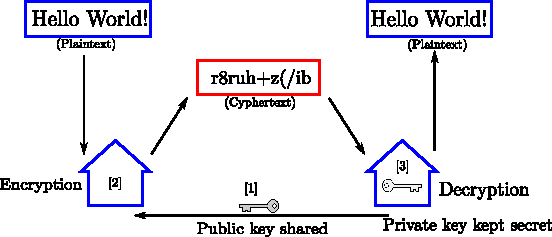
\includegraphics{asymmetrickey.pdf}
	\caption{In asymmetric key cryptography the plain-text is encoded, $[2]$, using the public key sent by the receiver, $[1]$, then sent as cypher-text to be decrypted with the private key which stays with the receiver at all times $[3]$.\label{fig:asymmetric-key}}
\end{figure}

This has proved to be an extremely secure method of sending data and is currently used by many banks and other industries to pass information and data with a minimum possibility of a breach of security. However, it is not impenetrable. Since the encryption and decryption keys must match each other, it is theoretically possible to calculate what the decryption key must be if one has the encryption one. As well as this, there is always the brute force method, which simply involves trying every possible combination of arrangements of the code to unlock the data until the correct one is found by elimination. Though this was unthinkable a few years sago, because of the size of the keys used, modern computers and networks of computers working together are starting to have the capabilities to break into these locked safes of information.

This is where quantum cryptography is different. Instead of having a key with more and more digits, hoping that this will make the lock more and more difficult to guess the correct key, quantum cryptography employs the Heisenberg Uncertainty Principle. The uncertainty principle states, in one of its forms, that:
\begin{quote}
	It is impossible to measure simultaneously both the position and velocity (or momentum) of a microscopic particle with absolute accuracy or certainty.
\end{quote}
This can be extended to the measurement when it takes place, observing the fact that the inaccuracies are introduced into the system, so that the principle can be stated as:
\begin{quote}
	It is not possible to measure or observe a particle system without disturbing that particle or system in some way.
\end{quote}

Analysis of this principle shows that there is another important rule of quantum mechanics here, that an arbitrary quantum state can not be copied exactly since this would involve first knowing the exact state of the system that was to be copied. This is important since it means that any attempt to eavesdrop on any information transfer can be detected as soon as the data is received.

\subsubsection{BB84}
We will examine the most commonly investigated method of quantum cryptography called BB84, so called after its inventors, Charles Bennett and Giles Brassard and the year they developed it, 1984\cite{DBLP:journals/joc/BennettBBSS92}.

The principle of sending quantum encoded information is fairly simple. The key that locks the information to be sent is encoded as qubits of light using the polarisation in the vertical and horizontal directions and the left and right diagonal directions to be either a ``0'' or ``1''. These are called baseis, the first is the rectilinear basis, the second is the diagonal basis. A third possibility is the circular basis where the polarisation is either right- or left-handed.

The key is sent to the receiver using one of the two settings randomly. For each value of the qubit, a different direction is defined, for example the arrangement shown in table~\ref{tab:basis}.
\begin{table}[h!t]
	\centering
	\begin{tabular}{c|c|c}
		Basis & 0 & 1 \\ \hline
		$+$ & $\uparrow$ & $\rightarrow$ \\
		$\times$ & $\nearrow$ & $\searrow$
	\end{tabular}
	\caption{\label{tab:basis}One possible arrangement of the two baseis $+$ and $\times$ and their corresponding qubit encoding.}
\end{table}

The sender creates a random bit and then selects one of the basis sets to encode it in. This is repeated for each bit in the set. For each qubit sent, the sender takes note of the randomly selected basis.

The receiver then makes measurements randomly of the qubits that have been sent using two analysers that detect if the qubit is polarised in the vertical/horizontal direction, or the diagonal direction. The sender does not reveal which direction setting was used to encode the ``0''s and ``1''s, meaning that the receiver and so also any eavesdropper does not know either. When the receiver measures the information, quantum uncertainty means that half of the time the right answer is found. This is due to the baseis not being orthogonal to each other and so a quantum measurement cannot determine between them. After the measurement, the photon is left in the state that it was measured to be in so an eavesdropper would affect the data being sent. 

The receiver does not know how the data was encoded so can at most only select at random which basis set to assign each qubit measured. After the information has been received, the sender releases the settings for the analyser so that the receiver knows which basis set was used for each individual qubit. The receiver can then correctly pick out the key from the results. On average, the correct value will have been found half of the time and the measurements where the correct answer is not found are discarded. The remaining bits constitute the shared key that the two parties can use, knowing that no-one else can have intercepted the transmission of the key.

\begin{table}[h!]
	\centering
	\begin{tabular}{r*{8}{c}}
		Sender's random bit & 1 & 0 & 1 & 0 & 0 & 1 & 1 & 1 \\
		Sender's random sending basis & $+$ & $+$ & $\times$ & $\times$ & $+$ & $+$ & $\times$ & $+$ \\
		Polarisation sent & $\rightarrow$ & $\uparrow$ & $\searrow$ & $\nearrow$ & $\uparrow$ & $\rightarrow$ & $\searrow$ & $\rightarrow$ \\
		Receiver's random measuring basis & $+$ & $\times$ & $\times$ & $+$ & $+$ & $\times$ & $+$ & $+$ \\
		Polarisation receiver measures & $\rightarrow$ & $\nearrow$ & $\searrow$ & $\rightarrow$ & $\uparrow$ & $\nearrow$ & $\rightarrow$ & $\rightarrow$ \\ 
		The settings are shared by the sender\\
		Shared secret key & 1 &  & 1 &  & 0 &  &  & 1
	\end{tabular}
\end{table}

\begin{figure}[ht]
	\centering
	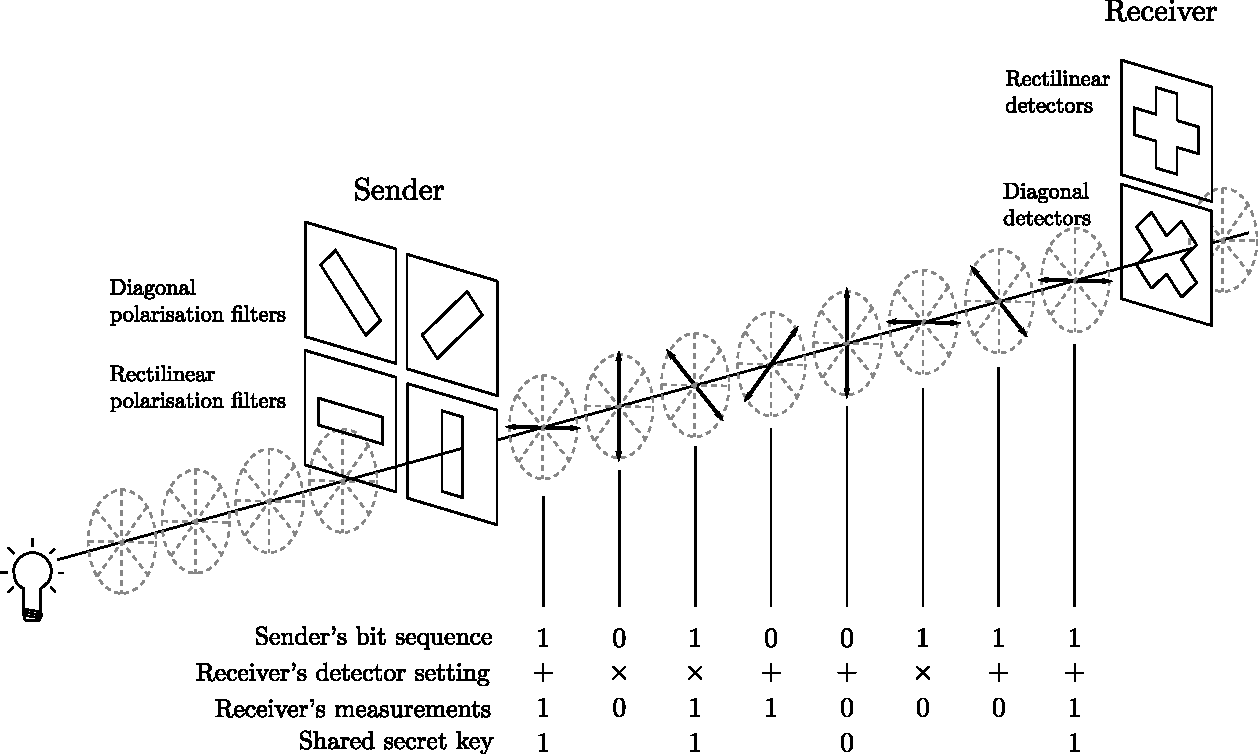
\includegraphics[width=1.0\columnwidth]{quantumcrypto.pdf}
	\caption{Using two different polarisation baseis to send a set of qubits securely\cite{quantumcrypto}.\label{fig:quantumcrypto}}
\end{figure}

One of the first experimental demonstrations of quantum cryptography was carried out in 2000 by a group at the University of Vienna using pairs of entangled photons\cite{PhysRevLett.84.4729}. They transmitted the encoded qubits over a distance of 360\,m via an optical fibre showing that the principle is definitely possible. However, the errors in transmission and measurement meant that they were unable to extend the distance the data was transferred. In 2004 though, another group from Toshiba Research at Cambridge managed to securely encode, transfer and decode a still image over a distance of 122\,km via a standard Telecom cable\cite{gobby:3762}. Figure~\ref{fig:quantumimage} shows the images that was transferred as well as the two keys that were generated and the decoded image. The small remaining errors in the image can be seen as defects to the colour, but overall, the image is very clearly the same as was transmitted.

\begin{figure}[ht]
	\centering
	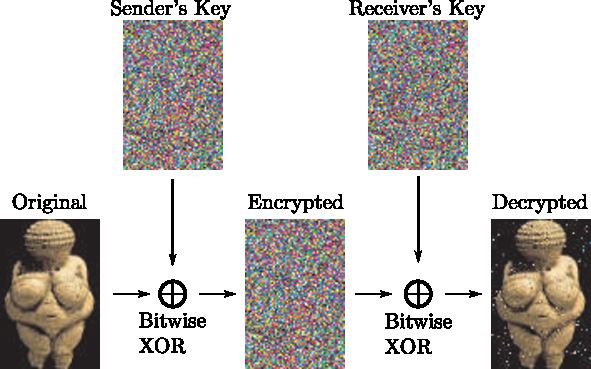
\includegraphics[width=0.7\columnwidth]{effigy.pdf}
	\caption{An image of the ``Venus von Willendorf'' effigy was transferred via a standard Telecom cable using polarised photon qubits and quantum cryptographic encoding.\label{fig:quantumimage}}
\end{figure}
